\documentclass[a4paper,12pt]{report}
\usepackage[top=2.5cm, bottom=2.5cm, left=2.5cm, right=2.5cm]{geometry}
\usepackage[czech]{babel}
\usepackage{setspace}
\usepackage{lmodern}
\usepackage{amsmath}
\usepackage{amsfonts}
\usepackage{amssymb}
\usepackage{amsthm}
\usepackage{graphicx}
\usepackage{wrapfig}
\usepackage{color}
\usepackage{xcolor}
\usepackage{url}
\usepackage{textcomp}
\usepackage{parskip}
\usepackage{tocloft}
\usepackage[bottom, perpage]{footmisc}


\usepackage[autostyle]{csquotes}

\usepackage{fontspec}
\setmainfont{Linux Libertine O}

\usepackage[ddmmyyyy]{datetime}
\renewcommand{\dateseparator}{.}

\setmainfont{Latin Modern Roman}
\setsansfont{Latin Modern Sans}
\setmonofont{Latin Modern Mono}

\setcounter{tocdepth}{3}
\setcounter{secnumdepth}{3}

\title{Take Your Pill}
\author{Vojtěch Hořánek}

\renewcommand{\baselinestretch}{1.5}

\pagenumbering{gobble}

\begin{document}

% Uzlabina title page
\begin{titlepage}
    \large
    \centering
    \vspace*{\fill}
    {\LARGE Take Your Pill}
    \vskip 1mm
    {\Large mobilní aplikace}
    \vskip1cm
    {\large SPŠE V Úžlabině}
    \vskip 20pt
    
\includegraphics[width=4cm]{uzlabina.png}
    \vskip 40pt
    Vojtěch Hořánek \\
    I4.D
    \vskip 15pt
    \today
    \vfill
\end{titlepage}


% Cestne prohlaseni
\vspace*{\fill}
\enquote{Prohlašuji, že jsem tuto práci vypracoval samostatně a použil jsem literárnı́ch pramenů a informacı́, které cituji a uvádı́m v seznamu použité literatury a zdrojů informacı́.}\hfill \break
V Praze dne
{
  \addfontfeature{LetterSpace=20.0}
  ....................\hfill....................
}
\begin{flushright}
    \setstretch{0.5}
    podpis autora
\end{flushright} 

% konec podpisu

% anotace
\newpage
\section*{Anotace}
Předložená práce je mobilní aplikace pro systém Android, která slouží k připomínání užití léků. V aplikaci je implementovaná historie připomínání a užívání léků, statistiky a grafy. Uživatel snadno získá přehled, jaké a kdy léky vynechává a může si nastavit opakované připomínání, aby již lék nezmeškal. Design aplikace je udělán tak, aby odpovídal material designu a jeho nejnovějším trendům. Aplikace je napsána v jazyce Kotlin a využívá moderních knihoven a technologií.
\vspace*{\fill}
\section*{Anotation}
The presented work is a mobile application for the Android operating system which reminds its users to take their pills. History, statistics, and graphs are implemented in the application. The user can effortlessly get an overview of which pills at what time did they miss and can set repeating reminders, so they do not forget them the next time. The application follows the material design guidelines and its latest trends. Kotlin was used as the programming language and utilizes modern libraries and technologies.

% konec anotace

\renewcommand\cftsecafterpnum{\vskip10pt}
\renewcommand\cftsubsecafterpnum{\vskip10pt}
\renewcommand\cftsubsubsecafterpnum{\vskip10pt}
\newpage
\tableofcontents % obsah

\chapter*{Úvod}
\addcontentsline{toc}{chapter}{Úvod}  

Cílem této práce bylo vytvořit aplikaci, která uživatelům usnadní pravidelné užívání léků jejich připomínáním, sledováním historie a statistik. Pro každý lék lze nastavit počet dní, po který se má připomínat, popř. počet dní, které vynechat, než se začne připomínat znovu a počet takovýchto cyklů.

Práce se skládá z mobilní aplikace pro systém android. Aplikace je navržena co nejjednodušeji a rozdělena do dvou hlavních sekcí: léky a historie. V sekci \enquote{léky} uživatel nalezne léky, které si do aplikace přidal. V jejich seznamu je zobrazen jejich název, popis, barva, fotografie a časy připomínek. V sekci \enquote{historie} může uživatel sledovat užití svých léku, zobrazí se mu kompletní historie (včetně kdy a jestli si lék vzal, kdy mu byla poslána připomínka a kolik prášků si vzal) a grafy zobrazující souhrnné informace. Součástí práce je i propagační a informační plakát. 

\pagenumbering{arabic} % start page numbering on Úvod


\chapter{Návrh aplikace}

Design aplikace jsem navrhoval před samotnou implementací, nutno ale dodat, že při implementaci prošel design několika iteracemi. Aplikaci jsem původně koncipoval jako jedinou hlavní obrazovku, kde by se uživateli ukázali všechny důležité informace. Postupem času se toto řešení ukázalo jako nevhodné a nepraktické, zvolil jsem proto více tradiční postup a to rozdělení aplikace do tří přehledných sekcí: \emph{Léky}, \emph{Historie} a \emph{Nastavení}. Každá obrazovka obsahuje velký nadpis a teprve potom samotný obsah. Mimo spodních dialogů\footnote{myšleno BottomSheetDialogFragment} není nadpis nijak ohraničen, pouze je odsazen. Změny mezi různými obrazovkami doprovázejí animace, které jsou implementovány podle Material Designu. Aplikace díky těmto animacím vypadá svižněji.

Celé rozhraní jsem upravil pomocí vlastních stylů, které vycházejí ze stylů Material Design \cite{materialdesign}. Pro některé prvky aplikace, jmenovitě titulky a tlačítka, jsem použil písmo \emph{Jost} \cite{jost}. Ikony použité v aplikaci jsou z knihovny Material Design Icons \cite{icons}, ikonu aplikace jsem získal od Austina Andrewse \cite{pill-icon} a grafika léků je dostupná na GitHubu pod názvem \emph{material-icons} \cite{pills-icons}. Nechybí ani podpora světlého a tmavého designu, který se dá přepínat v nastavení (VOJTO TODO REFERENCE).

\chapter{Implementace aplikace}

Při vytváření aplikace jsem vycházel ze zadání a využil jsem vlastních znalostní a zkušeností. Na naprogramování aplikace jsem použil programovací jazyk Kotlin. Zvolil jsem ho proto, že je preferovaný společností Google a oproti jazyku Java má mnoho výhod. Mnoho android knihoven vychází právě pro jazyk Kotlin a tak mi jeho použití ulehčilo mnoho práce při programování. Jmenovitě knihovny z rodiny Android Jetpack \cite{jetpack} jsem použil hojně.

Uživatelské rozhraní aplikace je napsáno v jazyce XML. Pro jeho manipulaci jsem použil knihovny \emph{ViewBinding} \cite{viewbinding} a \emph{DataBinding} \cite{databinding}.

Při samotném vývoji jsem používal vývojové prostředí \emph{Android Studio} \cite{studio} a emulátor \emph{Android Emulator}.

Aplikace je napsána tak, aby odpovídala architektuře \textbf{MVVM}\footnote{Model-View-ViewModel}. Znamená to, že každá obrazovka má svůj \emph{ViewModel} a každá datová sekce má svůj \emph{Repozitář}. Tyto třídy jsou odděleny od samotných fragmentů a aktivit (mají vlastní životní cyklus).

\vspace{6pt}
\fbox{\begin{minipage}{\linewidth}
\textbf{ViewModel} je třída obsahující funkce a proměnné využívané jednou obrazovkou aplikace, žije déle, než samotná obrazovka a může využívat funkcí jako například \emph{ViewModelScope}.
\end{minipage}}


\fbox{\begin{minipage}{\linewidth}
\textbf{Repozitář} (repository) je třída, která shromažďuje data a nabízí je ve vhodné formě ostatním třídám (například může data uchovat v mezipaměti). V této aplikaci přistupuje repozitář přímo do databáze a ve většině případů pouze volá funkce implementované v databázové vrstvě.
\end{minipage}}

\section{Uživatelské rozhraní}

Hlavní obrazovka\footnote{MainActivity} aplikace je rozdělena na tři části: \emph{Léky}, \emph{Historie} a \emph{Nastavení}. Uživatel mezi těmito sekcemi přepíná pomocí prvku \emph{BottomNavigationView}. Do sekce \emph{Historie} a na obrazovku \emph{Přidat lék} se může uživatel dostat i pomocí zkratky\footnote{App Shortcuts} z domovské obrazovky. Celá aplikace obsahuje pouze tři aktivity: MainActivity, AboutActivity a AppIntroActivity. Všechny ostatní obrazovky jsou implementovány jako fragmenty a pro jejich navigaci byla použita knihovna \emph{Navigation} \cite{navigation}

\subsection{Úvodní obrazovka}

Pro přidání úvodní obrazovky jsem použil knihovnu \emph{material-intro} \cite{intro}. Tato knihovna se postará o všechen layout a logiku úvodní obrazovky. Má jednoduché API a tak jediné, co jsem do aplikace přidal, byla aktivita \emph{AppIntroActivity} dědící ze třídy \emph{IntroActivity} a v ní přidal slidy pomocí funkce \emph{addSlide()}. Obrázky ve slidech jsem vyfotil v android emulátoru a upravil v programu \emph{GIMP}. Úvodní obrazovka se spustí pouze když uživatel aplikaci spustí poprvé. Toto je zajištěno tak, že do trvalé paměti aplikace\footnote{SharedPrefs} se po ukončení této aktivity uloží proměnná \emph{firstRun} s hodnotou \emph{false}.

\begin{figure}[h]
    \centering
    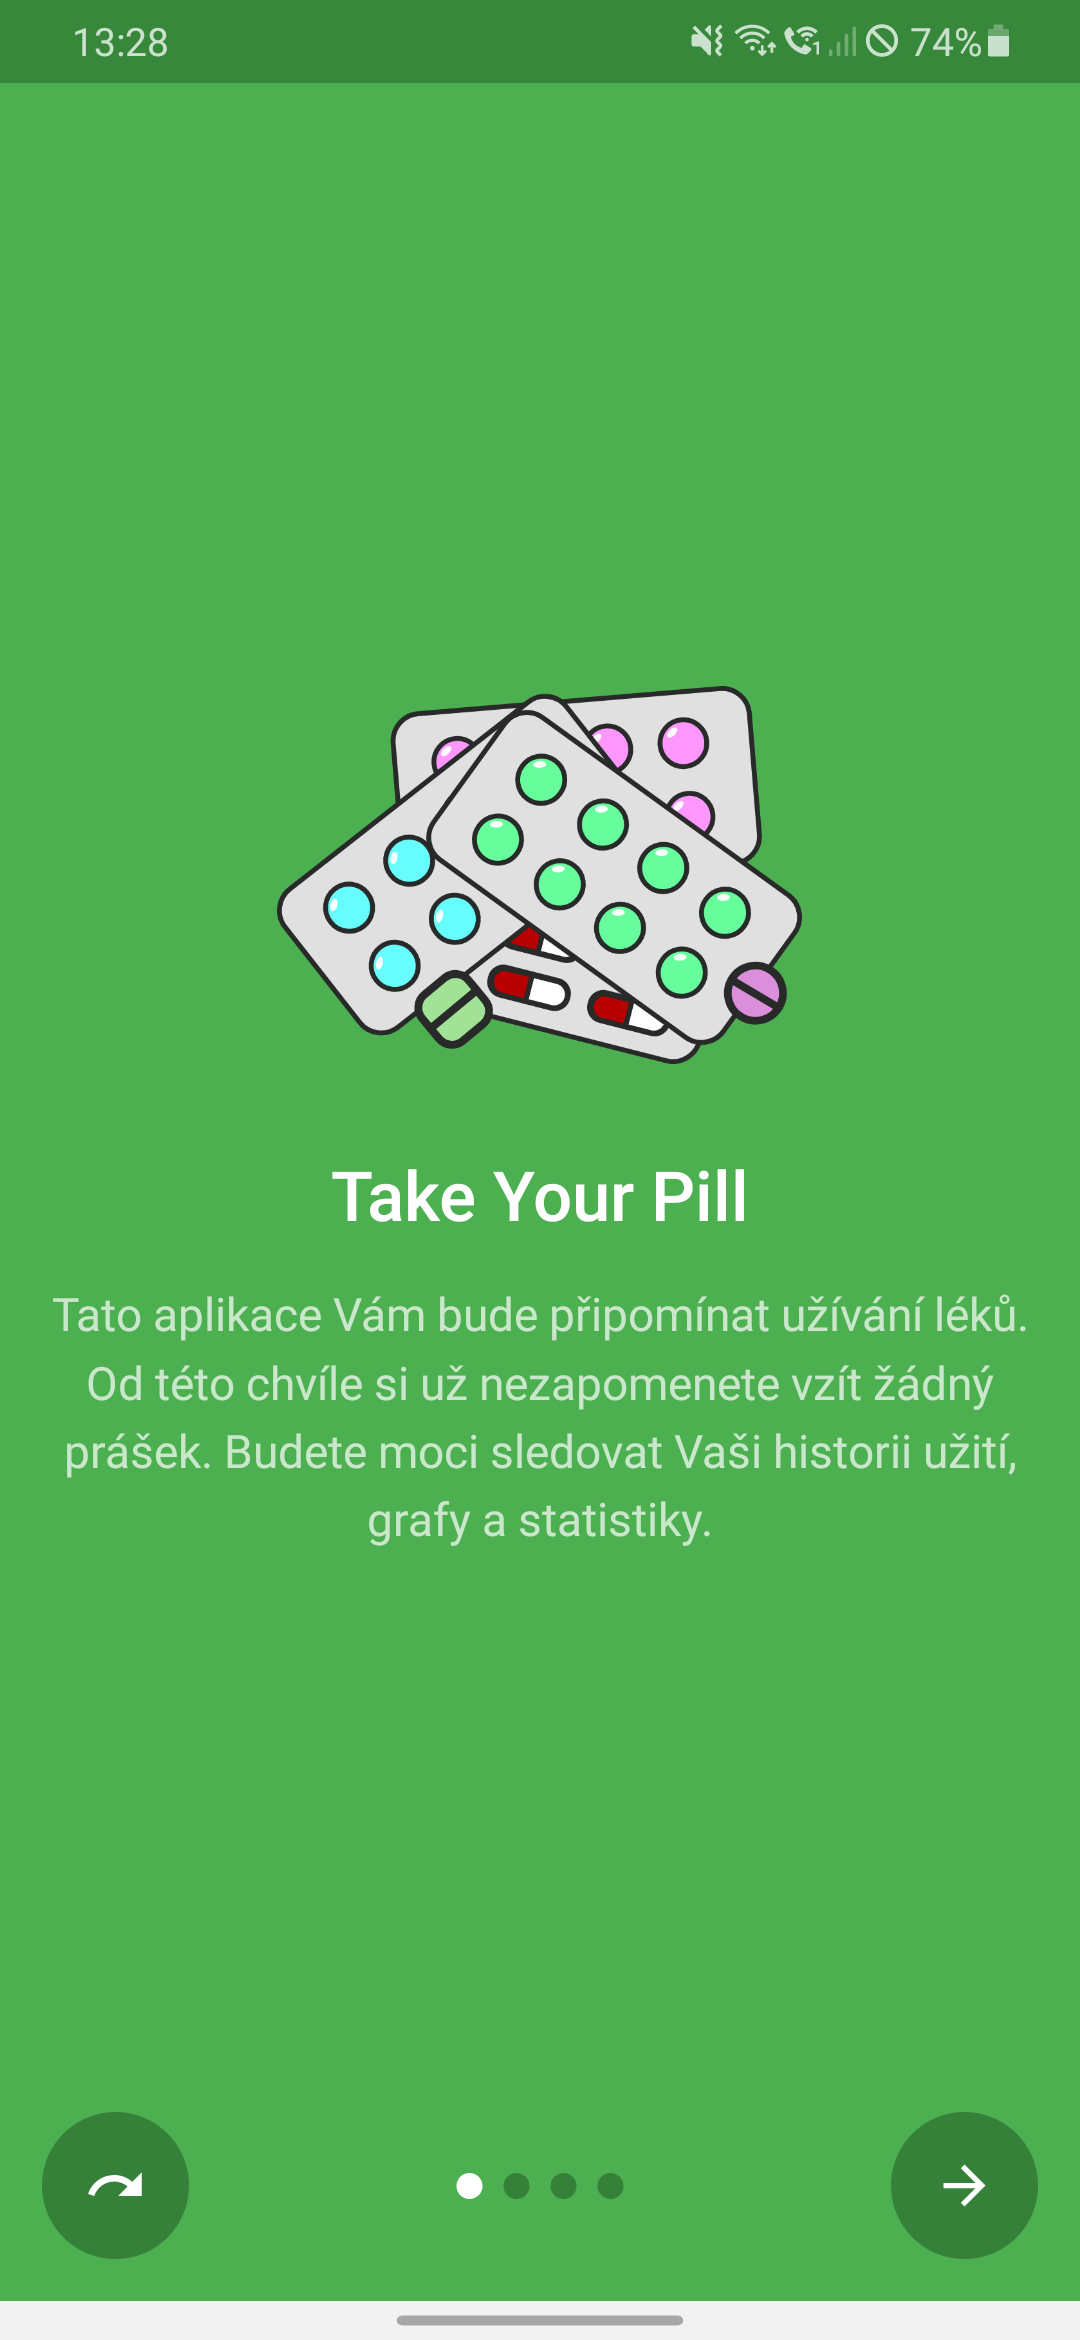
\includegraphics[width=0.3\textwidth]{app-intro-screenshot}
    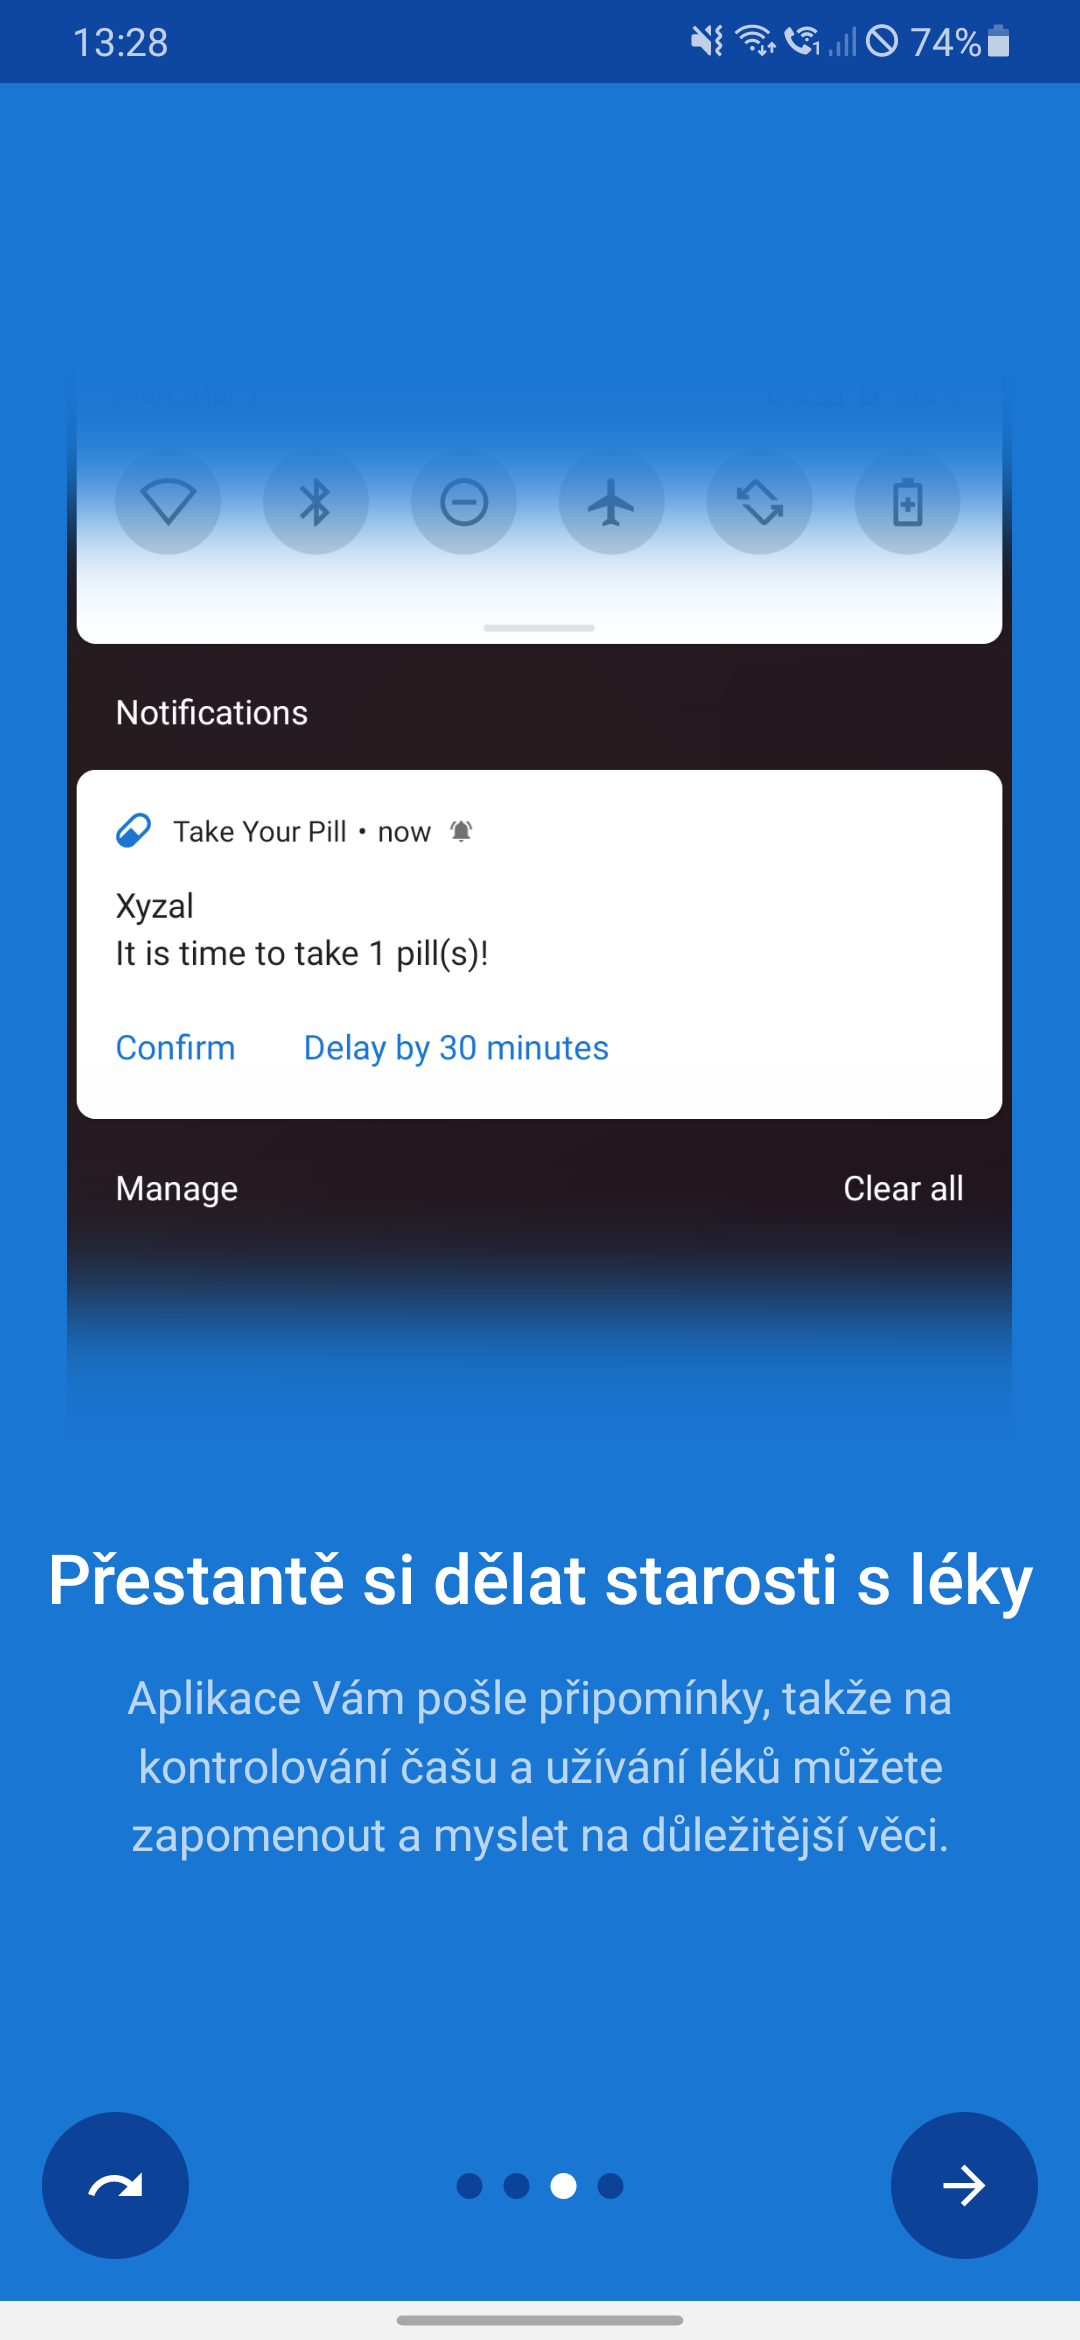
\includegraphics[width=0.3\textwidth]{app-intro-screenshot-2}
    \caption{Úvodní obrazovka}
\end{figure}


\subsection{Domovská obrazovka}
\subsubsection{Nový lék}
\subsubsection{Detail léku}
\subsection{Historie}
\subsubsection{Přehled}
\subsubsection{Grafy}
\subsection{Nastavení}
\subsubsection{O aplikaci}
\section{Programová implementace}
\subsection{Databáze}
\subsection{Připomínání}

\chapter*{Závěr}
\addcontentsline{toc}{chapter}{Závěr}  

\renewcommand\bibname{Bibliografie}
\begin{thebibliography}{9}

\bibitem{viewbinding} 
View Binding
\\\texttt{https://developer.android.com/topic/libraries/view-binding}

\bibitem{databinding} 
Data Binding Library
\\\texttt{https://developer.android.com/topic/libraries/data-binding}

\bibitem{materialdesign} 
Material Design
\\\texttt{https://material.io/design}

\bibitem{jetpack} 
Android Jetpack
\\\texttt{https://developer.android.com/jetpack}

\bibitem{studio} 
Android Studio
\\\texttt{https://developer.android.com/studio}

\bibitem{navigation} 
Navigation
\\\texttt{https://developer.android.com/guide/navigation}


\bibitem{intro} 
material-intro
\\\texttt{https://github.com/heinrichreimer/material-intro}

\bibitem{jost} 
Jost - Google Fonts
\\\texttt{https://fonts.google.com/specimen/Jost}


\bibitem{icons} 
Material Design Icons
\\\texttt{https://material.io/resources/icons/}

\bibitem{pill-icon} 
pill - Austin Andrews
\\\texttt{https://materialdesignicons.com/icon/pill}

\bibitem{pills-icons} 
ShimonHoranek - material-icons 
\\\texttt{https://github.com/ShimonHoranek/material-icons}



\end{thebibliography}

\end{document}
